%%%%%%%%%%%%%%%%%%%%%%%%%%%%%%%%%%%%%%%%%%%%%%%%%%%%%%%%%%%%%%%%%%%%%%
% LaTeX Example: Project Report
%
% Source: http://www.howtotex.com
%
% Feel free to distribute this example, but please keep the referral
% to howtotex.com
% Date: March 2011 
% 
%%%%%%%%%%%%%%%%%%%%%%%%%%%%%%%%%%%%%%%%%%%%%%%%%%%%%%%%%%%%%%%%%%%%%%
% How to use writeLaTeX: 
%
% You edit the source code here on the left, and the preview on the
% right shows you the result within a few seconds.
%
% Bookmark this page and share the URL with your co-authors. They can
% edit at the same time!
%
% You can upload figures, bibliographies, custom classes and
% styles using the files menu.
%
% If you're new to LaTeX, the wikibook is a great place to start:
% http://en.wikibooks.org/wiki/LaTeX
%
%%%%%%%%%%%%%%%%%%%%%%%%%%%%%%%%%%%%%%%%%%%%%%%%%%%%%%%%%%%%%%%%%%%%%%
% Edit the title below to update the display in My Documents
%\title{Project Report}
%
%%% Preamble
\documentclass[paper=a4, fontsize=10pt]{scrartcl}
\usepackage[T1]{fontenc}
\usepackage{fourier}
\usepackage{caption}
\usepackage[english]{babel}							% English language/hyphenation
\usepackage[protrusion=true,expansion=true]{microtype}	
\usepackage{amsmath,amsfonts,amsthm} % Math packages
\usepackage[pdftex]{graphicx}	
\usepackage{url}
\usepackage{wrapfig}
\usepackage{multirow}


\usepackage{sidecap}
%%% Custom sectioning
\usepackage{sectsty}
\allsectionsfont{\centering \normalfont\scshape}

\usepackage{geometry}
 \geometry{
 a4paper,
 total={210mm,297mm},
 left=10mm,
 right=10mm,
 top=10mm,
 bottom=10mm,
 }
%%% Custom headers/footers (fancyhdr package)
\usepackage{fancyhdr}
\pagestyle{fancyplain}
\fancyhead{}											% No page header
\fancyfoot[L]{}											% Empty 
\fancyfoot[C]{}											% Empty
\fancyfoot[R]{\thepage}									% Pagenumbering
\renewcommand{\headrulewidth}{0pt}			% Remove header underlines
\renewcommand{\footrulewidth}{0pt}				% Remove footer underlines
\setlength{\headheight}{13.6pt}


%%% Equation and float numbering
\numberwithin{equation}{section}		% Equationnumbering: section.eq#
\numberwithin{figure}{section}			% Figurenumbering: section.fig#
\numberwithin{table}{section}				% Tablenumbering: section.tab#


%%% Maketitle metadata
\newcommand{\horrule}[1]{\rule{\linewidth}{#1}} 	% Horizontal rule

\title{
		%\vspace{-1in} 	
		\usefont{OT1}{bch}{b}{n}
		\normalfont \normalsize \textsc{University Of Bristol / LaL Orsay} \\ [25pt]
		\horrule{0.5pt} \\[0.4cm]
		\huge Assessments \\
		\horrule{2pt} \\[0.5cm]
}
\author{
		\normalfont 								\normalsize
        Renato Quagliani\\[-3pt]		\normalsize
        \today
}
\date{}


%%% Begin document
\begin{document}
\maketitle
\section{Overview of work done}
A description of the work done up to now will be described. It consists in two major blocks. The first one which is related to the analysis work is a work done in between June 2014 and October 2014 , period in which i was finishing the master degree in Ferrara Unviersity and i get the NPAC master 2 at Paris Sud University. The second one is related to the work done in the context of the Upgrade of the LHCb detector consisting in the improvements of the \textit{Seeding} tracking algorithm which actually becomes the development of new algorithm , the \textit{Hybrid Seeding}.
The analysis work regards the study of double charm $B$ decays at \textit{LHCb} while the \textit{Seeding Algorithm for the LHCb upgrade} connsists in a software development project.
\subsection{Software development Project : Seeding Algorithm for the LHCb Upgrade}
Before discuss about the work done in this domain a small introduction about the tracking and the upgrade of the \textit{LHCb} detector is mandatory.
The data taking at \textit{LHCb} during 2011 and 2012 at LHCb are mainly determined by a few steps.
\begin{itemize}
\item{The \textit{L0 Trigger} which is implemented at the hardware level aiming to reduce the 40 \textit{MHz} bunch crossing rate to 1\textit{MHz} make use of estimation and measurements of the signature of particles having high $E_{T},p_{T}$. }. The main reason why this is done is because the read-out system as it is for Run-I and Run-II cannot affort an incoming rate of 40\textit{MHz}. In the upgrade all the reado-out will be substituted and the trigger will be done at the software level.
\item{\textit{High Level Trigger}: It consists in a software trigger where the tracking algorithms are run. During the Run-I, the seeding algorithm (called \textit{PatSeeding}) in the \textit{HLT} were runned making use of the left-over hits coming from the \textit{Forward} algorithm. During Run-I the \textit{Seeding} was used in the online reconstruction in tandem with the \textit{Forward} as described before while in the offline reconstruction it was run as a \textit{Standalone} algorithm. For the Run-II ...to complete.

The track reconstruction at \textit{LHCb} is decompose in different steps. The idea is to provide different containers containing different category of tracks. The track classification at \textit{LHCb} is done depending on the path the track goes through, so it's based on the datector's hit content as shown in Fig. ~\ref{figure:Tracks}.
\begin{figure}[h]
  \begin{center}
    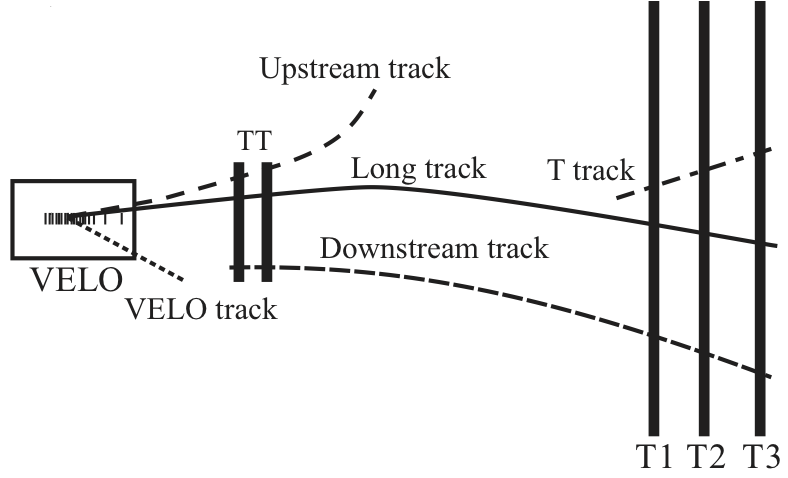
\includegraphics[width=0.5\textwidth]{Images/tracktype.png} 
  \caption{Track type at \textit{LHCb}. Velo tracks are basically straight lines since the magnetic field is almost 0 in that region. Tracks are mainly bended in the x-z\footnote{z- is the beam axis direction and the y axis is the B field line direction.} plane between the Tracker Turicensis (Upstream Tracker for the upgrade) and the T-Stations which is composed by the Inner Tracker(IT) and the Outer Tracker(OT) (Run-I and Run-II), while for the upgrade the stations will be replaced by the Scintillating Fibre tracker (SCIFI).}
  \label{figure:tracktype}
  \end{center}
\end{figure}
In the tracking system of \textit{LHCb} each track type is reconstructed by a proper algorithm and a schematic layout of how things works is given in table \ref{Table:tracks}.
\begin{table}[h]
\begin{tabular}{|l|l|l|l|l|}
\hline
Track Type & Used Detector &Algorithm(s)& Input&  Output    \\ \hline
\begin{tabular}[|l|]{@{}l@{}}Velo Tracks\\ or Velo-Segment\end{tabular} & Velo & Velo algorithm  & \multicolumn{1}{|l|}{/} & Velo         \\ \hline
\begin{tabular}[|l|]{@{}l@{}}Seed Tracks\\ or T-Tracks\end{tabular}     & \begin{tabular}[|l|]{@{}c@{}}T-Stations\\ (SciFi in upgrade)\end{tabular}                                                                                    & \multicolumn{1}{|l|}{Seeding algorithm}                                                                                             & \multicolumn{1}{|l|}{\begin{tabular}[|l|]{@{}l@{}}Allow the possible usage of\\ the leftover hits of forward.\\ If Not: Standalone Algorithm\end{tabular}} & Seed  \\ \hline
\multicolumn{1}{|l|}{\multirow{2}{*}{Long Tracks (1)}}                  & \multirow{2}{*}{\begin{tabular}[l]{@{}l@{}}Velo + TT + T-Stations\\ (TT $\rightarrow$ UT  \\ T-Stations $\rightarrow$ SciFi \\ in upgrade)\end{tabular}} & \begin{tabular}[|l|]{@{}l@{}} 1) Forward tracking:\\ Search in T-Stations knowing \\ Velo-Segment (adding also TT)\end{tabular}         & Velo Container               & \multirow{2}{*}{Long} \\ 
\multicolumn{1}{|l|}{}                                              &                                                                                                                                                            & \begin{tabular}[|l|]{@{}l@{}} 2)Matching algorithm:\\ Merge T-Tracks with Velo-Segment\\ 3)BestSelector= Forward+Matching\end{tabular} & Velo and Seed Containers                                                                                                                               &                       \\ \hline
Downstream Tracks                                                     & \multicolumn{1}{|l|}{\begin{tabular}[|l|]{@{}l@{}}T-Stations and TT\\ (SciFi and UT)\end{tabular}}                                                             & \begin{tabular}[|l|]{@{}l@{}}Downstream algorithm:\\ Use T-Tracks and\\ add TT (UT upgrade) hits\end{tabular}                         & Seed Container                                                                                                                                         & Downstream            \\ \hline Upstream Track                                                        & \multicolumn{1}{|l|}{Velo and TT} & \begin{tabular}[|l|]{@{}l@{}}Upstream algorithm:\\ Use Velo segment and \\ add TT( UT upgrade) hits\end{tabular} & Velo Container &  Upstream \\ \hline \end{tabular}
\end{table}

All the tracks produced by the algorithms provided before will be reprocessed by the Kalman Filter which will reprocess the tracks assigning a sort of \textit{univoque} $\chi^{2}$ to the track and will refit them taking into account the magnetic field map and the material budget of the tracks to multiscattering correction. From a more technical point of view, each track is defined by a vector of track state $\left( x, y, t_{x}, t_{y} , \frac{q}{p} \right)_{z}^{T}$ which is then propagated by a $5X5$ matrix through the detector considering the interactions and the B-Field map. At the level of the track search done by the algorithms the main goal is to provide for each track a set of compatible hits and only at the end of the algotithm they are converted into track state.

Going back to the upgrade, a brief description on what it consists is mandatory.


%\begin{itemize} 
%\item Velo tracks and Velo segments : tracks are reconstructed as 3-D object and they fill the container of \textit{Velo tracks} and they are found under the assumpiton that all of them originate from the same point.
%\item \textit{T-Tracks} , i.e., tracks going through the T-Station (\textit{SciFi} for upgrade) track reconstruction, it is done by the \textit{Seeding} algorithm and it runs as a standalone algorithm (alternitavely it can run on the leftover hits of the \textit{Forward} tracking). It's mainly useful to reconstruct tracks from long-lived particles such as $K_{s}^{0}$ and $\Lambda^{0}$  and in general tracks without \textit{Velo} segment. The \textit{seeding} algorithm ouput is used then to reconstruct \textit{Downstream} tracks, as well as \textit{long} tracks.
%\item \textit{Long} tracks, which are the most interesting one for physics analysis are reconstructed mainly by two algorithms : the \textit{Forward tracking} which took as input tracks from the \textit{Velo} and propagate them into the \textit{T-station} (\textit{SciFi}) adding also additional informations from the \textit{TT} (\textit{UT} for the upgrade). The second algorithm aiming to reconstruct \textit{Long} tracks is called \textit{Matching} and it combines the output of the \textit{Velo} algorithm and the output of the \textit{Seeding} algorithm.
%\item \textit{Upstream}  tracks are reconstructed throught the \textit{Upstrem} algorithm.
%\item Long 

\subsubsection{Analysis Work : $B^{0}\rightarrow D^{0}\overline{D}^{0}K^{\ast 0}$ analysis}
Nulla consequat massa quis enim. Donec pede justo, fringilla vel, aliquet nec, vulputate eget, arcu. In enim justo, rhoncus ut, imperdiet a, venenatis vitae, justo. Nullam dictum felis eu pede mollis pretium. Integer tincidunt. Cras dapibus. Vivamus elementum semper nisi. Aenean vulputate eleifend tellus. Aenean leo ligula, porttitor eu, consequat vitae, eleifend ac, enim.

\paragraph{Heading on level 4 (paragraph)}
Lorem ipsum dolor sit amet, consectetuer adipiscing elit. Aenean commodo ligula eget dolor. Aenean massa. Cum sociis natoque penatibus et magnis dis parturient montes, nascetur ridiculus mus. Donec quam felis, ultricies nec, pellentesque eu, pretium quis, sem. Nulla consequat massa quis enim. 


\section{Choice of Thesis Topic}

\begin{itemize}
	\item First item in a list 
          \begin{itemize}
          \item First item in a list 
            \begin{itemize}
            \item First item in a list 
            \item Second item in a list 
            \end{itemize}
          \item Second item in a list 
          \end{itemize}
	\item Second item in a list 
\end{itemize}

        \begin{enumerate}
	\item First item in a list 
	\item Second item in a list 
	\item Third item in a list
        \end{enumerate}
\section{Timetable for future}
%%% End document

\end{document}
